\begin{center}
    \textbf{--------- Lezione 4 - 7 ottobre 2020 ---------}
\end{center}

\section{Le notifiche push}
Nei protocolli di comunicazione abbiamo visto che è preferibile fare in modo che sia un’applicazione per dispositivi mobili a contattare un server e non viceversa. 
Ci sono però dei casi in cui non è possibile, se c'è un evento che si genera sul server, è il server stesso che deve contattare il client. 
\\ Ho diverse soluzioni:
\begin{itemize}
    \item mantenere una comunicazione aperta rispetto al server, ad esempio via TCP. 
    \\ Questa soluzione non va bene, è meglio evitare approcci connection-oriented
    \item il client rimane in attesa di connessione, esempio con un server socket. 
    Anche questa soluzione non va bene, il client non dovrebbe rimanere in ascolto di connessioni da parte del server
    \item il client fa polling: "hai qualche messaggio per me?"
    La soluzione non va bene in quanto sia costosa, dato che il client continua ad interrogare il server senza ricevere, nella maggior parte dei casi, nessun aggiornamento
    \item BOSH: permette al client di fare una richiesta HTTP al server e risponde subito se ha qualcosa. Se non ha niente, tiene la richiesta HTTP in attesa fino a quando non ha nulla da comunicare. 
    Può succedere che il client si disconnetta o che il client cambi IP. La richiesta fallisce e il client ne fa una nuova.
    Anche qui la soluzione richiede che il client sia sempre in esecuzione
\end{itemize}

C'è una soluzione ottimale, rispetto a quelle precedenti, che è quella delle \textit{notifiche push}. Si tiene un solo servizio attivo a livello di SO per ricevere comunicazioni asincrone. 
Questa soluzione fa in modo che sia il SO a rimanere in attesa di comunicazioni da un server esterno, dunque con una sola connessione, offrendo poi il servizio alle altre applicazioni. 

\subsection{Componenti delle notifiche}
Ci sono diverse componenti coinvolte:
\begin{itemize}
    \item l'\textbf{utente} che usa il dispositivo mobile
    \item \textbf{SO} del device
    \item \textbf{app} che deve ricevere la notifica
    \item \textbf{push server}, un servizio esterno che comunica con il SO (sviluppato da Apple e Google). Offre il servizio di push notification
    \item \textbf{app server}, un server che vuole inviare comunicazioni asincrone all'app
\end{itemize}

\subsection{Il protocollo}
Il protocollo alla base delle notifiche push è suddiviso in due fasi: setup e invio.

È necessario introdurre un elemento fondamentale del protocollo, il \textit{device token} che identifica la coppia data dal dispositivo e dell'applicazione ($<applicazione, device>$) che vuole ricevere le notifiche push. Il device token è creato dal push server usando tecniche crittografiche che garantiscono che il device token non possa essere creato da altri e che, una volta creato, non possa essere modificato.

\subsubsection{La fase di setup}
La fase di setup viene iniziata dall'app. Voglio permettere all'app server di mandare delle notifiche. 
Lo scopo è quindi quello di fare arrivare il device token all'app server. 
 
Il procedimento è il seguente.

\begin{figure}[!ht]
    \centering
    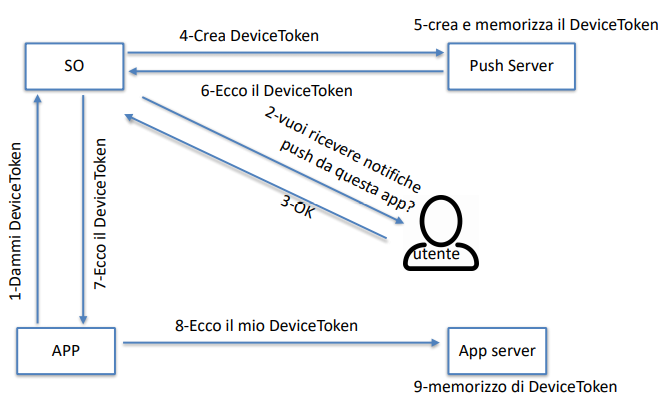
\includegraphics[width=.65\textwidth]{images/Mobile computing/3. Reti e architetture/setup.PNG}
\end{figure}

L'app fa una chiamata di API al SO che chiede all'utente se vuole autorizzare l'applicazione ad inviare le notifiche push. Se l'utente non autorizza, il procedimento finisce, se invece autorizza il SO chiede al Push Server di creare il DeviceToken. 
Il Push Server lo crea, lo memorizza e lo manda al SO. 
Il SO risponde all'app dando il DeviceToken. 

La richiesta "1. Dammi DeviceToken" è una chiamata bloccante oppure asincrona. 
L'app riceve il DeviceToken e lo comunica all'App server. 


\subsubsection{Fase di invio}
La fase di invio delle notifiche, invece, viene eseguita ogni volta che l’app server vuole mandare una comunicazione asincrona all’applicazione. 

Lo scopo è quindi di fare arrivare, tramite l'app server, all'app un messaggio con un piccolo payload. Il payload è il testo da mostrare ed eventuali altre informazioni come ad esempio "Hai 5 nuovi messaggi".

Il procedimento è il seguente. 
\begin{figure}[!ht]
    \centering
    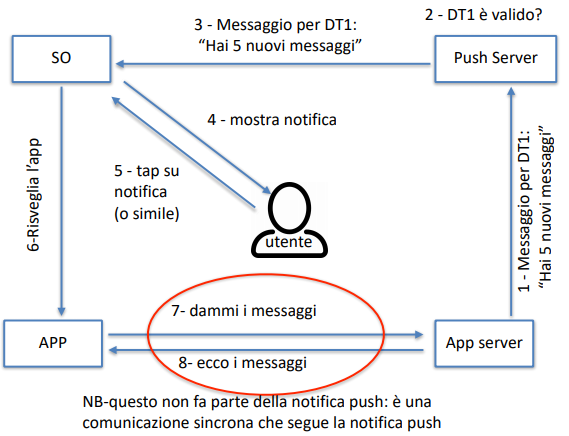
\includegraphics[width=.65\textwidth]{images/Mobile computing/3. Reti e architetture/invio.PNG}
\end{figure}

L'app server contatta il push server dicendo che ha un nuovo messaggio e allega due informazioni: il device token memorizzato in fase di setup e i payload. Il messaggio tra app server e push server è un messaggio tra due computer in rete. 
Il push server verifica che il device token sia valido e se è valido contatta il SO in modo asincrono, per esempio tramite l'implementazione di un protocollo simile a BOSH. Se il push server non riesce a contattare il SO, memorizza l'informazione della richiesta (ad esempio quando il telefono è spento o non ha connessione). 
Il SO mostra la notifica all'utente con anche il testo contenuto nel payload. L'utente fa il tap sulla notifica e il SO risveglia l'app.

\subsection{Attacchi}
Il protocollo alla base delle notifiche push fornisce garanzie di sicurezza più elevate rispetto ad altri servizi (ad esempio l'email).
Il push server può agire attivamente per prevenire gli attacchi. Alcuni esempi di attacchi che si possono prevenire sono:
\begin{itemize}
    \item \textbf{spamming}: un'app server non può inviare notifiche push ad un client che non lo ha autorizzato, perché non dispone del device token
    \item \textbf{impersonificazione}: un'app server non può far finta di essere un altro app server (es: telegram non può mandare una notifica push facendo finta di essere whatsapp). Questo aiuta a prevenire gli attacchi di tipo phishing (truffe) 
    \item \textbf{messaggi indesiderati}: se un app server inizia a mandare troppi messaggi o messaggi indesiderati all’utente, l’utente ha la possibilità di revocare il device token
    \item \textbf{flooding}: il push server può bloccare le richieste, se ad esempio un app server (anche autorizzato) prova ad inviarne un numero eccessivo allo stesso device
\end{itemize}

\subsection{Notifiche push e locali}
I SO rendono disponibili due tipi di notifiche: push e locali.
È facile fare confusione perché sono presentate in modo simile all'utente, ma sono completamente differenti da un punto di vista architetturale.
Le notifiche locali vengono generate dall'app stessa mediante delle chiamate al SO, di solito per dare informazioni all'utente quando l'app è in background (es: app di navigazione), oppure per mandare reminder all'utente ad orari prestabiliti.

